% ============================================================
%  Legal Case Outcome Prediction — Pipeline Progress Slides
%  Beamer: pdflatex updates_slides.tex
% ============================================================
\documentclass[aspectratio=169, 9pt]{beamer}

\usetheme{Madrid}
\usecolortheme{seahorse}
\setbeamertemplate{navigation symbols}{}
\setbeamertemplate{footline}[frame number]

\usepackage{booktabs}
\usepackage{tabularx}
\usepackage{multirow}
\usepackage{xcolor}
\usepackage{tikz}
\usetikzlibrary{arrows.meta, positioning, fit, backgrounds, shapes.geometric}
\usepackage{pgfplots}
\pgfplotsset{compat=1.18}
\usepackage{fontawesome5}
\usepackage{colortbl}
\usepackage{graphicx}
\usepackage{array}
\usepackage{makecell}

% ── colour palette ──────────────────────────────────────────
\definecolor{primary}{RGB}{25,55,109}
\definecolor{accent}{RGB}{220,80,50}
\definecolor{muted}{RGB}{100,120,150}
\definecolor{mygreen}{RGB}{30,140,80}
\definecolor{amber}{RGB}{200,130,0}
\definecolor{lightblue}{RGB}{230,240,255}
\definecolor{lstbg}{RGB}{245,245,245}
\definecolor{casecol}{RGB}{52,152,219}
\definecolor{seccol}{RGB}{39,174,96}
\definecolor{entcol}{RGB}{230,126,34}

\setbeamercolor{frametitle}{fg=white, bg=primary}
\setbeamercolor{title}{fg=white, bg=primary}
\setbeamercolor{block title}{bg=primary!90, fg=white}
\setbeamercolor{block body}{bg=lightblue}
\setbeamercolor{alerted text}{fg=accent}

% ── title ───────────────────────────────────────────────────
\title[Legal Case Outcome GNN]{%
  \textbf{Legal Case Outcome Prediction}\\[4pt]
  \large Pipeline \& Methodology Update}
\subtitle{NLP · Graph Construction · GNN Training · Benchmarking}
\author{Ziv Baretto}
\date{\today}

% ============================================================
\begin{document}
% ============================================================

\begin{frame}
  \titlepage
\end{frame}

\begin{frame}{Outline}
  \tableofcontents
\end{frame}

% ============================================================
\section{Input Data}
% ============================================================

\begin{frame}{Input Data — Raw Legal Case Corpus}
  \begin{columns}[T]
    \begin{column}{0.40\textwidth}
      \begin{block}{Dataset Overview}
        \small
        \begin{itemize}\setlength\itemsep{2pt}
          \item \textbf{91,166 PDF} legal documents from Indian courts
          \item 5 legal domains — balanced corpus
          \item Format: PDF + extracted \texttt{.txt}
          \item Jurisdiction: Indian High Courts \& Supreme Court
        \end{itemize}
      \end{block}
      \vspace{6pt}
      \begin{block}{Domain Breakdown}
        \scriptsize\renewcommand{\arraystretch}{1.15}
        \begin{tabular}{lrr}
          \toprule
          \textbf{Domain} & \textbf{\#Cases} & \textbf{\%}\\
          \midrule
          Family \& Matrimonial & 15,805 & 17.3\%\\
          Financial Fraud       & 15,023 & 16.5\%\\
          Land \& Property      & 14,502 & 15.9\%\\
          Motor Accidents       & 15,281 & 16.8\%\\
          Sexual Offences       & 15,538 & 17.0\%\\
          \midrule
          \textbf{Total}        & \textbf{76,149} & \textbf{100\%}\\
          \bottomrule
        \end{tabular}
      \end{block}
    \end{column}
    \begin{column}{0.57\textwidth}
      \centering
      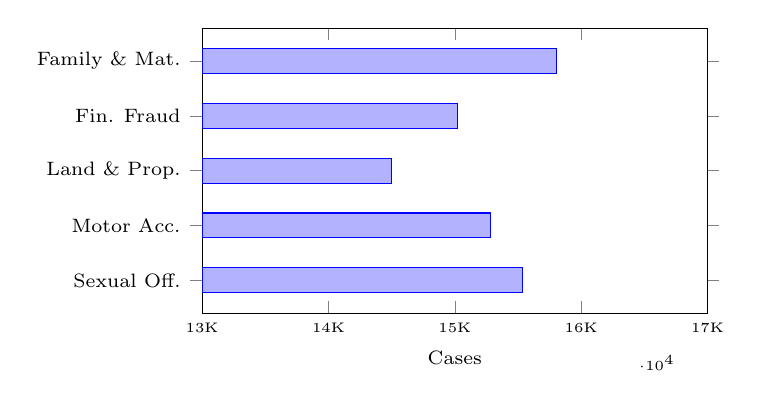
\begin{tikzpicture}
        \begin{axis}[
          xbar, bar width=9pt,
          xmin=13000, xmax=17000,
          width=8cm, height=5.2cm,
          symbolic y coords={
            {Sexual Off.},{Motor Acc.},{Land \& Prop.},{Fin. Fraud},{Family \& Mat.}},
          ytick=data,
          y tick label style={font=\scriptsize},
          x tick label style={font=\tiny},
          xlabel={\scriptsize Cases},
          xtick={13000,14000,15000,16000,17000},
          xticklabels={13K,14K,15K,16K,17K},
          every axis plot/.append style={fill=primary!65, draw=primary!90},
          enlarge y limits=0.15,
        ]
          \addplot coordinates {
            (15538,{Sexual Off.})
            (15281,{Motor Acc.})
            (14502,{Land \& Prop.})
            (15023,{Fin. Fraud})
            (15805,{Family \& Mat.})
          };
        \end{axis}
      \end{tikzpicture}
      \vspace{4pt}
      \begin{alertblock}{Key Challenge}
        \small Multi-hearing cases: one case can span months of hearings across multiple files — requires \textbf{deduplication \& timeline merging} before modelling.
      \end{alertblock}
    \end{column}
  \end{columns}
\end{frame}

% ============================================================
\section{NLP Preprocessing Pipeline}
% ============================================================

\begin{frame}{NLP Preprocessing — Three-Stage Pipeline}
  \centering
  \begin{tikzpicture}[
    node distance=0.55cm and 0.9cm,
    box/.style={draw=primary, fill=lightblue, rounded corners=4pt,
                minimum width=2.1cm, minimum height=1.1cm,
                align=center, font=\small},
    data/.style={draw=amber!80, fill=amber!15, rounded corners=3pt,
                 minimum width=1.7cm, minimum height=0.8cm,
                 align=center, font=\scriptsize},
    arr/.style={-{Stealth[length=6pt]}, thick, color=primary},
  ]
    \node[data] (pdfs) {91K PDFs\\\texttt{.txt} files};
    \node[box, right=of pdfs]  (ner)   {\faTag\ \textbf{NER + RR}\\OpenNyAI\\{\scriptsize 13 roles · 10 entities}};
    \node[box, right=of ner]   (summ)  {\faFileAlt\ \textbf{Summariser}\\OpenNyAI\\{\scriptsize Decision text}};
    \node[box, right=of summ]  (llm)   {\faRobot\ \textbf{LLM Label}\\Mistral/vLLM\\{\scriptsize 3 outcomes}};
    \node[box, right=of llm]   (merge) {\faCodeBranch\ \textbf{Timeline\\Merge}\\{\scriptsize 38.6K cases}};
    \node[data, right=of merge] (out)  {Enriched\\Case JSON};

    \draw[arr] (pdfs)--(ner);
    \draw[arr] (ner)--(summ);
    \draw[arr] (summ)--(llm);
    \draw[arr] (llm)--(merge);
    \draw[arr] (merge)--(out);
  \end{tikzpicture}

  \vspace{8pt}
  \begin{columns}[T]
    \begin{column}{0.30\textwidth}
      \begin{block}{\small \faTag\ Step 1: NER + RR}
        \scriptsize
        \textbf{Rhetorical Roles (13):}\\
        PREAMBLE · FAC · ISSUE\\
        ARG\_PET · ARG\_RESP\\
        PRE\_RELIED · RATIO · \ldots\\[4pt]
        \textbf{NER Entities (10):}\\
        COURT · JUDGE · STATUTE\\
        PROVISION · PRECEDENT · \ldots
      \end{block}
    \end{column}
    \begin{column}{0.30\textwidth}
      \begin{block}{\small \faFileAlt\ Step 2: Summariser}
        \scriptsize
        Extractive summarisation per rhetorical section (FAC, ANALYSIS, RATIO\ldots).\\[4pt]
        \texttt{decision} section text passed downstream to LLM.\\[4pt]
        Multi-GPU parallel; resume support.
      \end{block}
    \end{column}
    \begin{column}{0.36\textwidth}
      \begin{block}{\small \faRobot\ Step 3: LLM Outcome Label}
        \scriptsize
        Mistral (local vLLM) classifies outcome from \texttt{decision} summary + RPC-tagged sentences:\\[4pt]
        \textbf{Allowed} · \textbf{Dismissed} · \textbf{Allowed-in-part}\\[4pt]
        Confidence stored as \texttt{case\_outcome\_score}.
      \end{block}
    \end{column}
  \end{columns}
\end{frame}

% ============================================================
\section{Dataset Construction \& Timeline Merging}
% ============================================================

\begin{frame}{Timeline Merging — Multi-Hearing Consolidation}
  \begin{columns}[T]
    \begin{column}{0.48\textwidth}
      \begin{block}{Problem}
        \small One case $\to$ many JSON files (one per hearing date).\\
        GNN requires \textbf{one node per case} — all hearings must be merged.
      \end{block}
      \vspace{5pt}
      \begin{block}{Algorithm — \texttt{merge\_cases\_v2.py}}
        \small
        \begin{enumerate}\setlength\itemsep{2pt}
          \item \textbf{Group} files by case name
          \item \textbf{Dedup same-date:} keep file with most sentences
          \item \textbf{Containment check:} sample 20 chunks (150 chars each);\\
                if $\geq$60\% of older file exists in newest $\Rightarrow$ skip it
          \item \textbf{Append} unique content with separator:\\
                {\scriptsize\texttt{=== [HEARING: date] ===}}
          \item \textbf{Recalculate} all character offsets
        \end{enumerate}
      \end{block}
      \vspace{5pt}
      \begin{alertblock}{Result}
        \small 91,166 raw PDFs $\;\longrightarrow\;$ \textbf{38,645 merged cases}
      \end{alertblock}
    \end{column}
    \begin{column}{0.48\textwidth}
      \begin{block}{Post-Merge Dataset}
        \scriptsize\renewcommand{\arraystretch}{1.2}
        \begin{tabular}{lr}
          \toprule
          \textbf{Domain} & \textbf{Cases}\\
          \midrule
          Family \& Matrimonial & 15,307\\
          Financial Fraud       & 14,616\\
          Land \& Property      &  4,447\\
          Motor Accidents       &  4,274\\
          Sexual Offences       & (processing)\\
          \midrule
          \textbf{Total} & \textbf{38,645}\\
          \bottomrule
        \end{tabular}
      \end{block}
      \vspace{8pt}
      \centering
      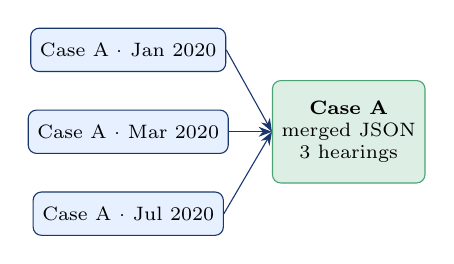
\begin{tikzpicture}[scale=0.8, every node/.style={font=\scriptsize}]
        \node[draw=primary, fill=lightblue, rounded corners=3pt,
              minimum width=1.6cm, minimum height=0.55cm, align=center]
          (f1) at (0, 1.3) {Case A · Jan 2020};
        \node[draw=primary, fill=lightblue, rounded corners=3pt,
              minimum width=1.6cm, minimum height=0.55cm, align=center]
          (f2) at (0, 0)   {Case A · Mar 2020};
        \node[draw=primary, fill=lightblue, rounded corners=3pt,
              minimum width=1.6cm, minimum height=0.55cm, align=center]
          (f3) at (0,-1.3) {Case A · Jul 2020};
        \node[draw=mygreen!80, fill=mygreen!15, rounded corners=3pt,
              minimum width=1.8cm, minimum height=1.3cm, align=center]
          (m) at (3.5, 0) {\textbf{Case A}\\merged JSON\\3 hearings};
        \draw[-{Stealth}, color=primary] (f1.east) -- (m.west);
        \draw[-{Stealth}, color=primary] (f2.east) -- (m.west);
        \draw[-{Stealth}, color=primary] (f3.east) -- (m.west);
      \end{tikzpicture}
    \end{column}
  \end{columns}
\end{frame}

% ============================================================
\section{Graph Construction — Reasoning-Focused Case-Star GNN}
% ============================================================

\begin{frame}{Graph Architecture — Reasoning-Focused Star Graph}
  \begin{columns}[T]
    \begin{column}{0.44\textwidth}
      \begin{block}{Core Design}
        \small Each case is a \textbf{star subgraph}: the case node at centre connected to typed \textbf{section nodes} (preamble, facts, arguments) and \textbf{shared entity nodes} (statutes, judges, courts).\\[5pt]
        Shared entities \textbf{link cases together} across the global graph.
      \end{block}
      \vspace{5pt}
      \begin{alertblock}{No Shortcut Edges}
        \small GNN must route \emph{through} argument nodes — forces reasoning about \emph{how} statutes/precedents were argued, not just \emph{which} ones appear.
      \end{alertblock}
      \vspace{5pt}
      \begin{block}{Scale (Financial Fraud)}
        \scriptsize\renewcommand{\arraystretch}{1.1}
        \begin{tabular}{lr}
          Cases              & 8,819\\
          Global nodes       & 134,214\\
          Node types         & 17\\
          Edge relation types & 42\\
          Avg edges / case   & $\approx$40\\
        \end{tabular}
      \end{block}
    \end{column}
    \begin{column}{0.53\textwidth}
      \centering
      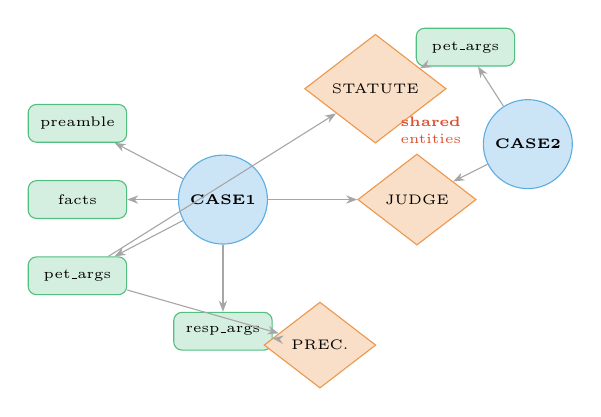
\begin{tikzpicture}[
        scale=0.88,
        case/.style={circle, draw=casecol!80, fill=casecol!25,
                     minimum size=0.85cm, font=\tiny\bfseries},
        sec/.style={rounded corners=3pt, draw=seccol!80, fill=seccol!20,
                    minimum width=1.25cm, minimum height=0.48cm,
                    align=center, font=\tiny},
        ent/.style={diamond, aspect=1.3, draw=entcol!80, fill=entcol!25,
                    minimum size=0.75cm, align=center, font=\tiny},
        arr/.style={-{Stealth[length=4pt]}, gray!70, thin},
        shr/.style={-{Stealth[length=4pt]}, accent, thick},
      ]
        % ── Case 1 ──
        \node[case] (c1) at (0,0) {CASE\\1};
        \node[sec]  (pre)  at (-2.1, 1.1) {preamble};
        \node[sec]  (fac)  at (-2.1, 0.0) {facts};
        \node[sec]  (apet) at (-2.1,-1.1) {pet\_args};
        \node[sec]  (are)  at ( 0.0,-1.9) {resp\_args};

        \draw[arr] (c1)--(pre);
        \draw[arr] (c1)--(fac);
        \draw[arr] (c1)--(apet);
        \draw[arr] (c1)--(are);

        % ── Shared entities ──
        \node[ent] (stat) at (2.2, 1.6)  {\tiny STATUTE};
        \node[ent] (judg) at (2.8, 0.0)  {\tiny JUDGE};
        \node[ent] (prec) at (1.4,-2.1)  {\tiny PREC.};

        \draw[arr] (apet)--(stat);
        \draw[arr] (apet)--(prec);
        \draw[arr] (are) --(prec);
        \draw[arr] (c1)  --(judg);

        % ── Case 2 (shares entities) ──
        \node[case] (c2) at (4.4, 0.8) {CASE\\2};
        \node[sec]  (apet2) at (3.5, 2.2) {pet\_args};

        \draw[arr] (c2)--(apet2);
        \draw[arr] (apet2)--(stat);
        \draw[arr] (c2)--(judg);

        % ── "Shared" label ──
        \node[font=\tiny, color=accent, align=center] at (3.0, 1.0)
          {\textbf{shared}\\entities};
      \end{tikzpicture}

      \vspace{4pt}
      {\scriptsize
        \textcolor{casecol}{$\bullet$}~Case node\quad
        \textcolor{seccol}{$\blacksquare$}~Section node\quad
        \textcolor{entcol}{$\blacklozenge$}~Shared entity}
    \end{column}
  \end{columns}
\end{frame}

% ────────────────────────────────────────────────────────────
\begin{frame}{Graph Node Types — 17 Types}
  \begin{columns}[T]
    \begin{column}{0.46\textwidth}
      \begin{block}{\small Document / Section Nodes \emph{(local to each case)}}
        \scriptsize\renewcommand{\arraystretch}{1.15}
        \begin{tabular}{lr}
          \toprule
          \textbf{Node Type} & \textbf{Count}\\
          \midrule
          \texttt{case}                     & 8,819\\
          \texttt{preamble}                 & 8,819\\
          \texttt{facts}                    & 7,325\\
          \texttt{arguments}                & 7,092\\
          \texttt{petitioner\_arguments}    & 6,261\\
          \texttt{respondent\_arguments}    & 3,803\\
          \texttt{other\_lawyer\_arguments} & 3,154\\
          \bottomrule
        \end{tabular}\\[4pt]
        Each sourced from the corresponding rhetorical role label (RR).
      \end{block}
    \end{column}
    \begin{column}{0.50\textwidth}
      \begin{block}{\small Shared Entity Nodes \emph{(cross-case)}}
        \scriptsize\renewcommand{\arraystretch}{1.15}
        \begin{tabular}{lr}
          \toprule
          \textbf{Node Type} & \textbf{Count}\\
          \midrule
          \texttt{precedent}          & 20,082\\
          \texttt{respondent}         & 13,642\\
          \texttt{lawyer}             & 13,236\\
          \texttt{petitioner}         & 12,853\\
          \texttt{provision}          &  6,960\\
          \texttt{court}              &  3,228\\
          \texttt{statute}            &  2,542\\
          \texttt{judge}              &  1,624\\
          \texttt{petitioner\_lawyer} &    649\\
          \texttt{defence\_lawyer}    &    193\\
          \bottomrule
        \end{tabular}
      \end{block}
      \vspace{4pt}
      \begin{block}{\small Excluded Entity Types}
        \scriptsize
        \texttt{ORG} · \texttt{GPE} · \texttt{DATE} · \texttt{CASE\_NUMBER}\\
        Too noisy or non-causal for legal reasoning.
      \end{block}
    \end{column}
  \end{columns}
\end{frame}

% ────────────────────────────────────────────────────────────
\begin{frame}{Graph Edge Types — 42 Relations}
  \begin{columns}[T]
    \begin{column}{0.46\textwidth}
      \begin{block}{\small Case $\to$ Section Edges}
        \scriptsize\renewcommand{\arraystretch}{1.1}
        \begin{tabular}{ll}
          \toprule
          \textbf{From} & \textbf{To (relation)}\\
          \midrule
          \texttt{case} & \texttt{preamble} (has\_preamble)\\
          \texttt{case} & \texttt{facts} (has\_facts)\\
          \texttt{case} & \texttt{arguments}\\
          \texttt{case} & \texttt{petitioner\_arguments}\\
          \texttt{case} & \texttt{respondent\_arguments}\\
          \texttt{case} & \texttt{other\_lawyer\_arguments}\\
          \bottomrule
        \end{tabular}
      \end{block}
      \vspace{4pt}
      \begin{block}{\small Case $\to$ Party / Court}
        \scriptsize\renewcommand{\arraystretch}{1.1}
        \begin{tabular}{ll}
          \toprule
          \textbf{From} & \textbf{To (relation)}\\
          \midrule
          \texttt{case} & \texttt{petitioner} / \texttt{respondent}\\
          \texttt{case} & \texttt{court} (heard\_in)\\
          \texttt{case} & \texttt{judge} (decided\_by\_bench)\\
          \texttt{case} & \texttt{lawyer} / \texttt{pet\_lawyer} / \texttt{def\_lawyer}\\
          \bottomrule
        \end{tabular}
      \end{block}
    \end{column}
    \begin{column}{0.50\textwidth}
      \begin{block}{\small Argument $\to$ Citation Edges}
        \scriptsize\renewcommand{\arraystretch}{1.1}
        \begin{tabular}{ll}
          \toprule
          \textbf{From} & \textbf{To (relation)}\\
          \midrule
          \texttt{arguments} & \texttt{precedent} (cites\_precedent)\\
          \texttt{arguments} & \texttt{statute} (cites\_statute)\\
          \texttt{arguments} & \texttt{provision} (cites\_provision)\\
          \texttt{provision} & \texttt{statute} (belongs\_to)\\
          \bottomrule
        \end{tabular}
      \end{block}
      \vspace{4pt}
      \begin{block}{\small Lawyer $\to$ Argument (role-specific)}
        \scriptsize\renewcommand{\arraystretch}{1.1}
        \begin{tabular}{ll}
          \toprule
          \textbf{From} & \textbf{To}\\
          \midrule
          \texttt{petitioner\_lawyer} & \texttt{petitioner\_arguments}\\
          \texttt{defence\_lawyer}    & \texttt{respondent\_arguments}\\
          \texttt{lawyer}             & \texttt{other\_lawyer\_arguments}\\
          \texttt{petitioner}         & \texttt{petitioner\_arguments}\\
          \texttt{respondent}         & \texttt{respondent\_arguments}\\
          \bottomrule
        \end{tabular}
      \end{block}
      \vspace{4pt}
      \begin{alertblock}{\small Bidirectional}
        \scriptsize All relations are bidirectional (\texttt{use\_to\_undirected: true}) $\Rightarrow$ \textbf{42 total edge types}.
      \end{alertblock}
    \end{column}
  \end{columns}
\end{frame}

% ────────────────────────────────────────────────────────────
\begin{frame}{Removed Edges — Enforcing Reasoning Paths}
  \begin{columns}[T]
    \begin{column}{0.42\textwidth}
      \begin{block}{Deliberately Removed Shortcuts}
        \scriptsize\renewcommand{\arraystretch}{1.2}
        \begin{tabular}{p{3.0cm}p{2.8cm}}
          \toprule
          \textbf{Removed edge} & \textbf{Why removed}\\
          \midrule
          \texttt{statute/provision}\\$\to$ \texttt{arguments}
            & Must route via typed arg nodes\\[4pt]
          \texttt{judge}\\$\to$ \texttt{arguments}
            & Prevent judge-outcome shortcut\\[4pt]
          \texttt{petitioner/respondent}\\$\to$ \texttt{arguments}
            & Must use role-specific nodes\\[4pt]
          \texttt{all lawyers}\\$\to$ \texttt{arguments}
            & Lawyer attribution must be role-specific\\
          \bottomrule
        \end{tabular}
      \end{block}
      \vspace{4pt}
      \begin{alertblock}{Effect}
        \small GNN must aggregate \textbf{argument-context features} before forming any case representation.
      \end{alertblock}
    \end{column}
    \begin{column}{0.54\textwidth}
      \centering
      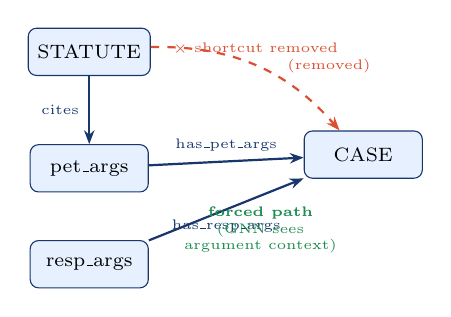
\begin{tikzpicture}[
        scale=0.87,
        n/.style={draw=primary, fill=lightblue, rounded corners=3pt,
                  minimum width=1.5cm, minimum height=0.6cm,
                  align=center, font=\scriptsize},
        arr/.style={-{Stealth[length=5pt]}, thick, primary},
        bad/.style={-{Stealth[length=5pt]}, thick, accent, dashed},
        lbl/.style={font=\tiny},
      ]
        \node[n] (stat)   at (0, 2.2) {STATUTE};
        \node[n] (petarg) at (0, 0.5) {pet\_args};
        \node[n] (rearg)  at (0,-0.9) {resp\_args};
        \node[n] (case)   at (4, 0.7) {CASE};

        % Good forced paths
        \draw[arr] (stat)   -- node[lbl,left]{cites}          (petarg);
        \draw[arr] (petarg) -- node[lbl,above]{has\_pet\_args}(case);
        \draw[arr] (rearg)  -- node[lbl,below]{has\_resp\_args}(case);

        % Bad shortcut
        \draw[bad, bend left=25] (stat) to
          node[lbl, above, color=accent]{$\times$~shortcut removed} (case);

        % Annotation
        \node[lbl, color=mygreen, align=center] at (2.5,-0.4)
          {\textbf{forced path}\\(GNN sees\\argument context)};
        \node[lbl, color=accent] at (3.5, 2.0) {(removed)};
      \end{tikzpicture}

      \vspace{6pt}
      {\small\color{muted}
        The statute must pass through the \textbf{argument node} —\\
        the model sees \emph{how} it was argued, not just that it appeared.}
    \end{column}
  \end{columns}
\end{frame}

% ────────────────────────────────────────────────────────────
\begin{frame}{Preventing Data Leakage — What Was Excluded \& Why}
  \begin{columns}[T]
    \begin{column}{0.50\textwidth}
      \begin{block}{Excluded from Node Text Features}
        \scriptsize\renewcommand{\arraystretch}{1.25}
        \begin{tabular}{p{2.2cm}p{4.0cm}}
          \toprule
          \textbf{Excluded} & \textbf{Why (leakage risk)}\\
          \midrule
          \texttt{RATIO} sentences
            & Ratio decidendi — states the court's binding conclusion.
              Directly encodes the outcome.\\
          \midrule
          \texttt{RPC} sentences (Rationale/ Principle Cited)
            & Court declares which legal principles it applies.
              Written \emph{after} the decision is reached.\\
          \midrule
          \texttt{PRE\_RELIED} / \texttt{PRE\_NOT\_RELIED} sentences
            & Which precedents the court adopted or rejected.
              Post-decision information — reveals winning side.\\
          \midrule
          \texttt{decision} summary field
            & Extractive summary of dispositional text (used only for LLM labelling).
              Never fed into GNN node features.\\
          \midrule
          \texttt{case\_outcome\_label} \& \texttt{case\_outcome\_score}
            & Target variable — kept strictly as label, never as feature.\\
          \bottomrule
        \end{tabular}
      \end{block}
    \end{column}
    \begin{column}{0.46\textwidth}
      \begin{block}{Rhetorical Role Timeline}
        \centering\vspace{4pt}
        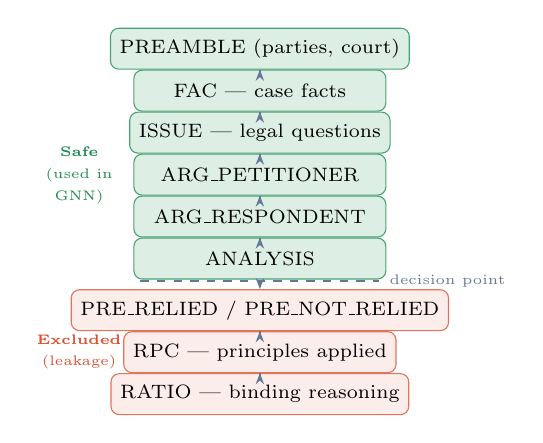
\begin{tikzpicture}[
          scale=0.82,
          every node/.style={font=\scriptsize},
          safe/.style={draw=mygreen!80, fill=mygreen!15, rounded corners=3pt,
                       minimum width=3.2cm, minimum height=0.52cm, align=center},
          leak/.style={draw=accent!80, fill=accent!10, rounded corners=3pt,
                       minimum width=3.2cm, minimum height=0.52cm, align=center},
          arr/.style={-{Stealth[length=4pt]}, thick, muted},
        ]
          \node[safe] (p1) at (0, 3.4)  {PREAMBLE (parties, court)};
          \node[safe] (p2) at (0, 2.75) {FAC — case facts};
          \node[safe] (p3) at (0, 2.1)  {ISSUE — legal questions};
          \node[safe] (p4) at (0, 1.45) {ARG\_PETITIONER};
          \node[safe] (p5) at (0, 0.8)  {ARG\_RESPONDENT};
          \node[safe] (p6) at (0, 0.15) {ANALYSIS};
          \draw[thick, dashed, muted] (-1.85,-0.2) -- (1.85,-0.2)
            node[right, font=\tiny, color=muted] {decision point};
          \node[leak] (q1) at (0,-0.65) {PRE\_RELIED / PRE\_NOT\_RELIED};
          \node[leak] (q2) at (0,-1.3)  {RPC — principles applied};
          \node[leak] (q3) at (0,-1.95) {RATIO — binding reasoning};

          \draw[arr] (p1)--(p2); \draw[arr] (p2)--(p3);
          \draw[arr] (p3)--(p4); \draw[arr] (p4)--(p5);
          \draw[arr] (p5)--(p6);
          \draw[arr] (p6.south) -- (q1.north);
          \draw[arr] (q1)--(q2); \draw[arr] (q2)--(q3);

          \node[font=\tiny, color=mygreen] at (-2.8, 1.8)  {\textbf{Safe}};
          \node[font=\tiny, color=mygreen] at (-2.8, 1.45) {(used in};
          \node[font=\tiny, color=mygreen] at (-2.8, 1.1)  {GNN)};
          \node[font=\tiny, color=accent]  at (-2.8,-1.1)  {\textbf{Excluded}};
          \node[font=\tiny, color=accent]  at (-2.8,-1.45) {(leakage)};
        \end{tikzpicture}
      \end{block}
      \vspace{4pt}
      \begin{alertblock}{Split Design}
        \scriptsize Cases split at \textbf{case level} (not sentence level) into train / val / test — no cross-case contamination through shared entity nodes.
      \end{alertblock}
    \end{column}
  \end{columns}
\end{frame}

% ============================================================
\section{Text Encoding — Multi-Encoder Benchmarking}
% ============================================================

\begin{frame}{Multi-Encoder Benchmarking Setup}
  \begin{columns}[T]
    \begin{column}{0.50\textwidth}
      \begin{block}{Four Encoders Compared}
        \scriptsize\renewcommand{\arraystretch}{1.2}
        \begin{tabular}{p{1.8cm}p{3.2cm}r}
          \toprule
          \textbf{Encoder} & \textbf{Model} & \textbf{Dim}\\
          \midrule
          \texttt{hashing}     & Feature hash (baseline)     & 384\\
          \texttt{bge\_m3}     & BAAI/bge-m3 (multilingual)  & 1024\\
          \texttt{inlegalbert} & law-ai/InLegalBERT          & 768\\
          \texttt{longformer}  & legal-xlm-longformer-base   & 768\\
          \bottomrule
        \end{tabular}
      \end{block}
      \vspace{5pt}
      \begin{block}{Controlled Experiment Design}
        \small\textbf{All other variables fixed:}
        \begin{itemize}\scriptsize\setlength\itemsep{1pt}
          \item Same graph topology (reasoning-focused)
          \item Same train/val/test case splits
          \item Same HGT architecture \& hyperparameters
          \item 3 random seeds per encoder: 42, 43, 44
        \end{itemize}
        \vspace{3pt}
        $\mathbf{4}$ encoders $\times$ $\mathbf{3}$ seeds $= \mathbf{12}$ total runs
      \end{block}
    \end{column}
    \begin{column}{0.46\textwidth}
      \begin{block}{HGT Architecture}
        \small
        \begin{tabular}{ll}
          \toprule
          Model    & Heterogeneous Graph Transformer\\
          \midrule
          Node types & 17 \quad Edge types: 42\\
          Input dim  & encoder dim + 12 (metadata)\\
          Task       & Node classification (case nodes)\\
          Labels     & Allowed / Dismissed / In-part\\
          Metric     & Macro-F1\\
          \bottomrule
        \end{tabular}
      \end{block}
      \vspace{5pt}
      \begin{block}{Node Features}
        \small Text embedding \textbf{+} structural metadata:
        \begin{itemize}\scriptsize\setlength\itemsep{2pt}
          \item Degree, node-type one-hot
          \item Connectivity rank within legal domain
        \end{itemize}
      \end{block}
      \vspace{5pt}
      \begin{alertblock}{Domain}
        \small Financial Fraud — 8,819 cases
      \end{alertblock}
    \end{column}
  \end{columns}
\end{frame}

% ────────────────────────────────────────────────────────────
\begin{frame}{Benchmark Results — BGE-M3 Wins}
  \begin{columns}[T]
    \begin{column}{0.50\textwidth}
      \begin{block}{Macro-F1 Results (avg over 3 seeds)}
        \scriptsize\renewcommand{\arraystretch}{1.3}
        \begin{tabular}{lrrrr}
          \toprule
          \textbf{Encoder} & \textbf{Val F1} & \textbf{Test F1} & \textbf{Epoch} & \textbf{$\sigma$}\\
          \midrule
          \rowcolor{mygreen!15}
          \textbf{bge\_m3}  & \textbf{0.7662} & \textbf{0.7513} & 55 & 0.014\\
          hashing (base)    & 0.7427 & 0.7401 & 37 & 0.008\\
          inlegalbert       & 0.7412 & 0.7345 & 56 & 0.002\\
          longformer        & 0.7378 & 0.7177 & 50 & 0.004\\
          \bottomrule
        \end{tabular}
      \end{block}
      \vspace{4pt}
      \centering
      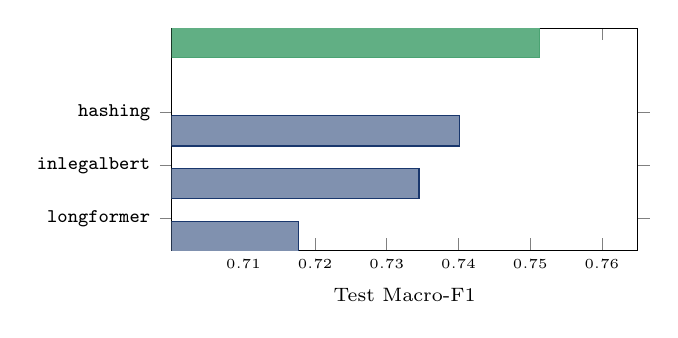
\begin{tikzpicture}
        \begin{axis}[
          xbar, bar width=11pt,
          xmin=0.70, xmax=0.765,
          width=7.5cm, height=4.4cm,
          symbolic y coords={longformer, inlegalbert, hashing, bge-m3},
          ytick=data,
          y tick label style={font=\scriptsize\ttfamily},
          x tick label style={font=\tiny},
          xlabel={\scriptsize Test Macro-F1},
          xtick={0.71,0.72,0.73,0.74,0.75,0.76},
          enlarge y limits=0.2,
        ]
          \addplot[fill=primary!55, draw=primary]
            coordinates {(0.7177,longformer)(0.7345,inlegalbert)(0.7401,hashing)};
          \addplot[fill=mygreen!70, draw=mygreen!80]
            coordinates {(0.7513,bge-m3)};
        \end{axis}
      \end{tikzpicture}
    \end{column}
    \begin{column}{0.46\textwidth}
      \begin{alertblock}{Key Finding}
        \textbf{BGE-M3} (multilingual, general-purpose) outperforms both legal domain-specific encoders.\\[4pt]
        Multilingual pretraining better captures \textbf{Indian legal English} than UK/US legal corpora.
      \end{alertblock}
      \vspace{6pt}
      \begin{block}{Notable Observations}
        \small
        \begin{itemize}\setlength\itemsep{3pt}
          \item \texttt{hashing} baseline \textbf{beats domain encoders} — graph structure alone carries strong signal
          \item \texttt{longformer} worst despite long-context design — nodes are short sentence spans, not documents
          \item BGE-M3 gain: $+2.4$\,pp val, $+1.1$\,pp test
          \item All runs stable ($\sigma \leq 0.014$); convergence in 37--56 epochs
        \end{itemize}
      \end{block}
      \vspace{4pt}
      \begin{block}{Conclusion}
        \small\textbf{BGE-M3 selected} for all subsequent experiments.
      \end{block}
    \end{column}
  \end{columns}
\end{frame}

% ============================================================
\section{Graph Visualiser}
% ============================================================

\begin{frame}{Interactive Graph Visualiser (Dash App)}
  \begin{columns}[T]
    \begin{column}{0.46\textwidth}
      \begin{block}{Two Complementary Views}
        \small
        \begin{enumerate}\setlength\itemsep{4pt}
          \item \textbf{Hub Network} — entity + case nodes.\\
                Colour = domain, size = degree.\\
                Reveals structurally central statutes, judges, courts.
          \item \textbf{Case Connection Network} — case-only graph, edges = shared legal entities.\\
                Thickness tiers: 1--2 / 3--5 / 6+ shared entities.
        \end{enumerate}
      \end{block}
      \vspace{5pt}
      \begin{block}{Interaction}
        \small
        Click node $\to$ right panel shows \textbf{connected cases} with exact bridge entities grouped by type.\\[3pt]
        Full-details modal: sorted tabular view; visual cap = top 50 highlighted; all in modal.
      \end{block}
      \vspace{5pt}
      \begin{block}{Graph Loaded}
        \scriptsize\renewcommand{\arraystretch}{1.1}
        \begin{tabular}{lr}
          Sample nodes & 4,897\\
          Sample edges & 10,292\\
          Case-case pairs & 49,149\\
          Domains & 5\\
        \end{tabular}
      \end{block}
    \end{column}
    \begin{column}{0.50\textwidth}
      \begin{block}{Technical Architecture}
        \small
        \begin{itemize}\setlength\itemsep{3pt}
          \item \textbf{Dash + Plotly} (WebGL Scattergl traces)
          \item Pre-built spring layouts (\texttt{layout.pkl}) — zero layout computation at runtime
          \item $\leq$8 Scattergl traces per view ensures reliable WebGL click detection
          \item Connectivity-ranked sampling: top-$N$ cases per domain by structural centrality
          \item Dashboard cards (top hubs, bridge nodes, stats) pre-rendered at startup
        \end{itemize}
      \end{block}
      \vspace{5pt}
      \begin{alertblock}{Cross-Domain Bridge Nodes}
        \small Entities linking $\geq$2 legal domains reveal cross-domain patterns — e.g.\ a statute cited in both fraud and land dispute cases.
      \end{alertblock}
      \vspace{5pt}
      \begin{block}{Key Engineering Fix}
        \scriptsize Grouping traces by \emph{node type only} (not node-type $\times$ bucket) reduced trace count from $\sim$49 to $\sim$8, fixing unreliable click detection in WebGL.
      \end{block}
    \end{column}
  \end{columns}
\end{frame}

% ============================================================
\section{Summary \& Pipeline Overview}
% ============================================================

\begin{frame}{End-to-End Pipeline}
  \centering
  \begin{tikzpicture}[
    scale=0.78, transform shape,
    node distance=0.28cm and 0.50cm,
    step/.style={draw=primary, fill=lightblue, rounded corners=4pt,
                 minimum width=1.85cm, minimum height=1.05cm,
                 align=center, font=\scriptsize},
    data/.style={draw=amber!80, fill=amber!15, rounded corners=3pt,
                 minimum width=1.6cm, minimum height=0.8cm,
                 align=center, font=\scriptsize},
    arr/.style={-{Stealth[length=5pt]}, thick, primary},
  ]
    \node[data] (raw)  {91K PDFs\\5 domains};
    \node[step, right=of raw]   (ner)   {\faTag\\\textbf{NER + RR}\\OpenNyAI\\13 roles};
    \node[step, right=of ner]   (summ)  {\faFileAlt\\\textbf{Summariser}\\OpenNyAI\\decision};
    \node[step, right=of summ]  (llm)   {\faRobot\\\textbf{LLM Label}\\Mistral\\3 classes};
    \node[step, right=of llm]   (merge) {\faCodeBranch\\\textbf{Merge}\\38.6K\\cases};
    \node[step, right=of merge] (graph) {\faSitemap\\\textbf{Graph\\Build}\\17 types};
    \node[step, right=of graph] (enc)   {\faCogs\\\textbf{Encode}\\BGE-M3\\1024-d};
    \node[step, right=of enc]   (hgt)   {\faBrain\\\textbf{HGT\\Train}\\3 seeds};
    \node[data, right=of hgt]   (out)   {Test F1\\0.7513};

    \draw[arr] (raw)--(ner); \draw[arr] (ner)--(summ);
    \draw[arr] (summ)--(llm); \draw[arr] (llm)--(merge);
    \draw[arr] (merge)--(graph); \draw[arr] (graph)--(enc);
    \draw[arr] (enc)--(hgt); \draw[arr] (hgt)--(out);
  \end{tikzpicture}

  \vspace{8pt}
  \begin{columns}
    \begin{column}{0.24\textwidth}
      \begin{block}{\centering\small Scale}
        \centering\scriptsize
        91K documents\\
        5 legal domains\\
        38.6K merged cases\\
        134K graph nodes
      \end{block}
    \end{column}
    \begin{column}{0.24\textwidth}
      \begin{block}{\centering\small NLP}
        \centering\scriptsize
        OpenNyAI NER/RR\\
        13 rhetorical roles\\
        Mistral LLM labels\\
        Containment merge
      \end{block}
    \end{column}
    \begin{column}{0.24\textwidth}
      \begin{block}{\centering\small Graph}
        \centering\scriptsize
        17 node types\\
        42 edge relations\\
        No shortcut edges\\
        Reasoning-first HGT
      \end{block}
    \end{column}
    \begin{column}{0.24\textwidth}
      \begin{block}{\centering\small Best Result}
        \centering\scriptsize
        BGE-M3 encoder\\
        Val F1: \textbf{0.7662}\\
        Test F1: \textbf{0.7513}\\
        Seed 42, epoch 55
      \end{block}
    \end{column}
  \end{columns}
\end{frame}

% ── Thank you ─────────────────────────────────────────────────
\begin{frame}[plain]
  \begin{center}
    \vspace{2cm}
    {\Large\bfseries\color{primary} Thank You}\\[16pt]
    {\large Questions \& Discussion}\\[24pt]
    \textcolor{muted}{\small
      NLP annotation $\to$ timeline merging $\to$ GNN graph construction $\to$ multi-encoder benchmarking $\to$ outcome prediction
    }
  \end{center}
\end{frame}

\end{document}
